\documentclass{zkdl-presentation-template}

% Bibliography
\usepackage[backend=biber]{biblatex}
\bibliography{refs.bib}

\usepackage{tabularx}

% Include subfigure package
\usepackage{subfigure}
\usepackage{subcaption}

\usepackage{bbm}

% Numeration
\addtobeamertemplate{navigation symbols}{}{%
    \usebeamerfont{footline}%
    \usebeamercolor[fg]{footline}%
    \hspace{1em}%
    \textbf{\insertframenumber/\inserttotalframenumber}
    \vspace{3.5px}
}

\title[Activation-Efficient Networks]{\textbf{Аналіз ефективних для активації архітектур нейронних мереж для задач машинного навчання}} 

\author{Виконав: Захаров Дмитро Олегович\inst{1} \\ Науковий керівник: Ігнатович Світлана Юріївна\inst{2}} 

\institute[shortinst]{
    \inst{1} Студент групи МП41 IV курсу (перший бакалаврський рiвень), спецiальностi 113
``Прикладна математика'' освiтньої програми ``Прикладна математика''.\\
    \inst{2} Доктор фiз.-мат. наук, професор кафедри прикладної математики.
}

\date{16 квітня 2025}

\begin{document}
    \frame {
      \titlepage 
      %\hfill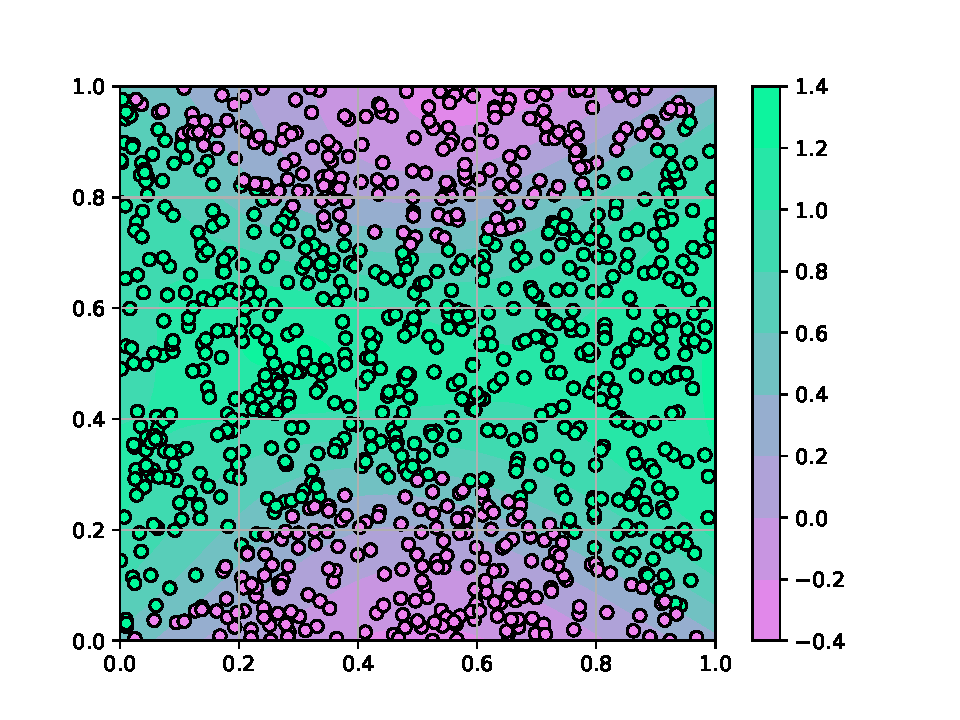
\includegraphics[trim={1.75cm 2.0cm 3.75cm 1cm},clip,width=0.4\textwidth]{../code/classification-cont-prediction.pdf}
    }
  
    \begin{frame}{План}
      \tableofcontents
    \end{frame}

    \section[Вступ]{Вступ}
    \begin{frame}{Причини}
        Зараз, використання нейронних мереж є стандартом у багатьох задачах
        машинного навчання.

        \begin{figure}
            \centering
            \begin{tikzpicture}[
                box/.style={
                    draw=blue!60!black,       % dark blue outline
                    fill=blue!20,             % light blue background
                    ultra thick, 
                    minimum width=1.8cm, 
                    minimum height=1.2cm, 
                    align=center
                },
                >=Stealth
              ]
            
              % Nodes
              \node[box, label={[yshift=0.7em]above:\small Neural Network}] (nn) {\large $f(\cdot;\theta)$};
              \node[left=2.5cm of nn] (input) {\large $x$};
              \node[right=2.5cm of nn] (output) {\large $y$};
            
              % Arrows
              \draw[->, thick] (input) -- (nn);
              \draw[->, thick] (nn) -- (output);
            
            \end{tikzpicture}
            \caption{Нейронна мережа є певною параметризованою функцією $f(\cdot;\theta)$, що
            перетворює вхідні дані $x$ у вихідні $y$.}
        \end{figure}

        Найбільш поширена архітектура --- це MLP (\textbf{M}ulti-\textbf{L}ayer
        \textbf{P}erceptron), що записується як:
        \begin{equation*}
            \boldsymbol{x}^{(\ell+1)} = \sigma(\boldsymbol{W}^{(\ell)}\boldsymbol{x}^{(\ell)} + \boldsymbol{b}^{(\ell)}), \quad \ell \in [L].
        \end{equation*}
        \vspace{-10px}
        В такому разі, $f(\boldsymbol{x}) = \boldsymbol{x}^{(L)}$ для $\boldsymbol{x}^{(0)} = \boldsymbol{x}$.
    \end{frame}

    \begin{frame}{Про силу нейронних мереж}
        \begin{tikzpicture}[scale=0.8]
            % Define layers and node style
            \tikzset{input-neuron/.style={
                circle, 
                draw=green!80!black, 
                line width=0.5mm,
                fill=green!20!white,
                minimum size=0.5cm
            }}
            \tikzset{hidden-neuron/.style={
                circle, 
                draw=blue!80!black, 
                line width=0.5mm,
                fill=blue!20!white,
                minimum size=0.5cm
            }}
            \tikzset{output-neuron/.style={
                circle, 
                draw=orange!80!black, 
                line width=0.5mm,
                fill=orange!20!white,
                minimum size=0.5cm
            }}
            
            % Input layer
            \foreach \i in {1, 2, 3} {
                \node[input-neuron] (I\i) at (0, -1.25*\i) {$x_{\i}$};
            }
        
            % Hidden layer
            \foreach \j in {1, 2, 3, 4, 5} {
                \node[hidden-neuron] (h\j) at (4, -1.25*\j + 1.25) {$\Sigma$};
                \node[hidden-neuron] (H\j) at (6, -1.25*\j + 1.25) {$z_{\j}$};
                \draw[very thick,-{Stealth[length=3.5mm]}] (h\j) to [edge label=$\sigma$] (H\j);
            }
        
            % Output layer
            \node[output-neuron] (O) at (10, -2.5) {$f(\boldsymbol{x})$};
        
            % Draw connections from input to hidden layer
            \foreach \i in {1, 2, 3} {
                \foreach \j in {1, 2, 3, 4, 5} {
                    \draw[very thick,-{Stealth[length=3.5mm]}] (I\i) -- (h\j);
                }
            }
        
            % Draw connections from hidden to output layer
            \foreach \j in {1, 2, 3, 4, 5} {
                \draw[very thick,-{Stealth[length=3.5mm]}] (H\j) -- (O);
            }
        
            % Labels
            \node[above, align=center] at (0, 0.5) {\textcolor{green!80!black}{\textbf{Вхідний шар}}\\$m$ нейронів};
            \node[above, align=center] at (5, 0.5) {\textcolor{blue!80!black}{\textbf{Прихований шар}}\\$n$ нейронів};
            \node[above, align=center] at (10, 0.5) {\textcolor{orange!80!black}{\textbf{Вихідний шар}}\\1 нейрон};
        
        \end{tikzpicture}

        \begin{theorem}[Universal Approximation Theorem]
            Якщо $\sigma$ \textcolor{orange!90!black}{не є поліномом} та $L \geq 2$, то $f$ є щільною в
            $L^{\infty}(K)$ для будь-якої компактної множини $K \subseteq
            \mathbb{R}^m$.
        \end{theorem}
    \end{frame}

    \begin{frame}{Безпека нейронних мереж}
        \begin{figure}
            \centering
            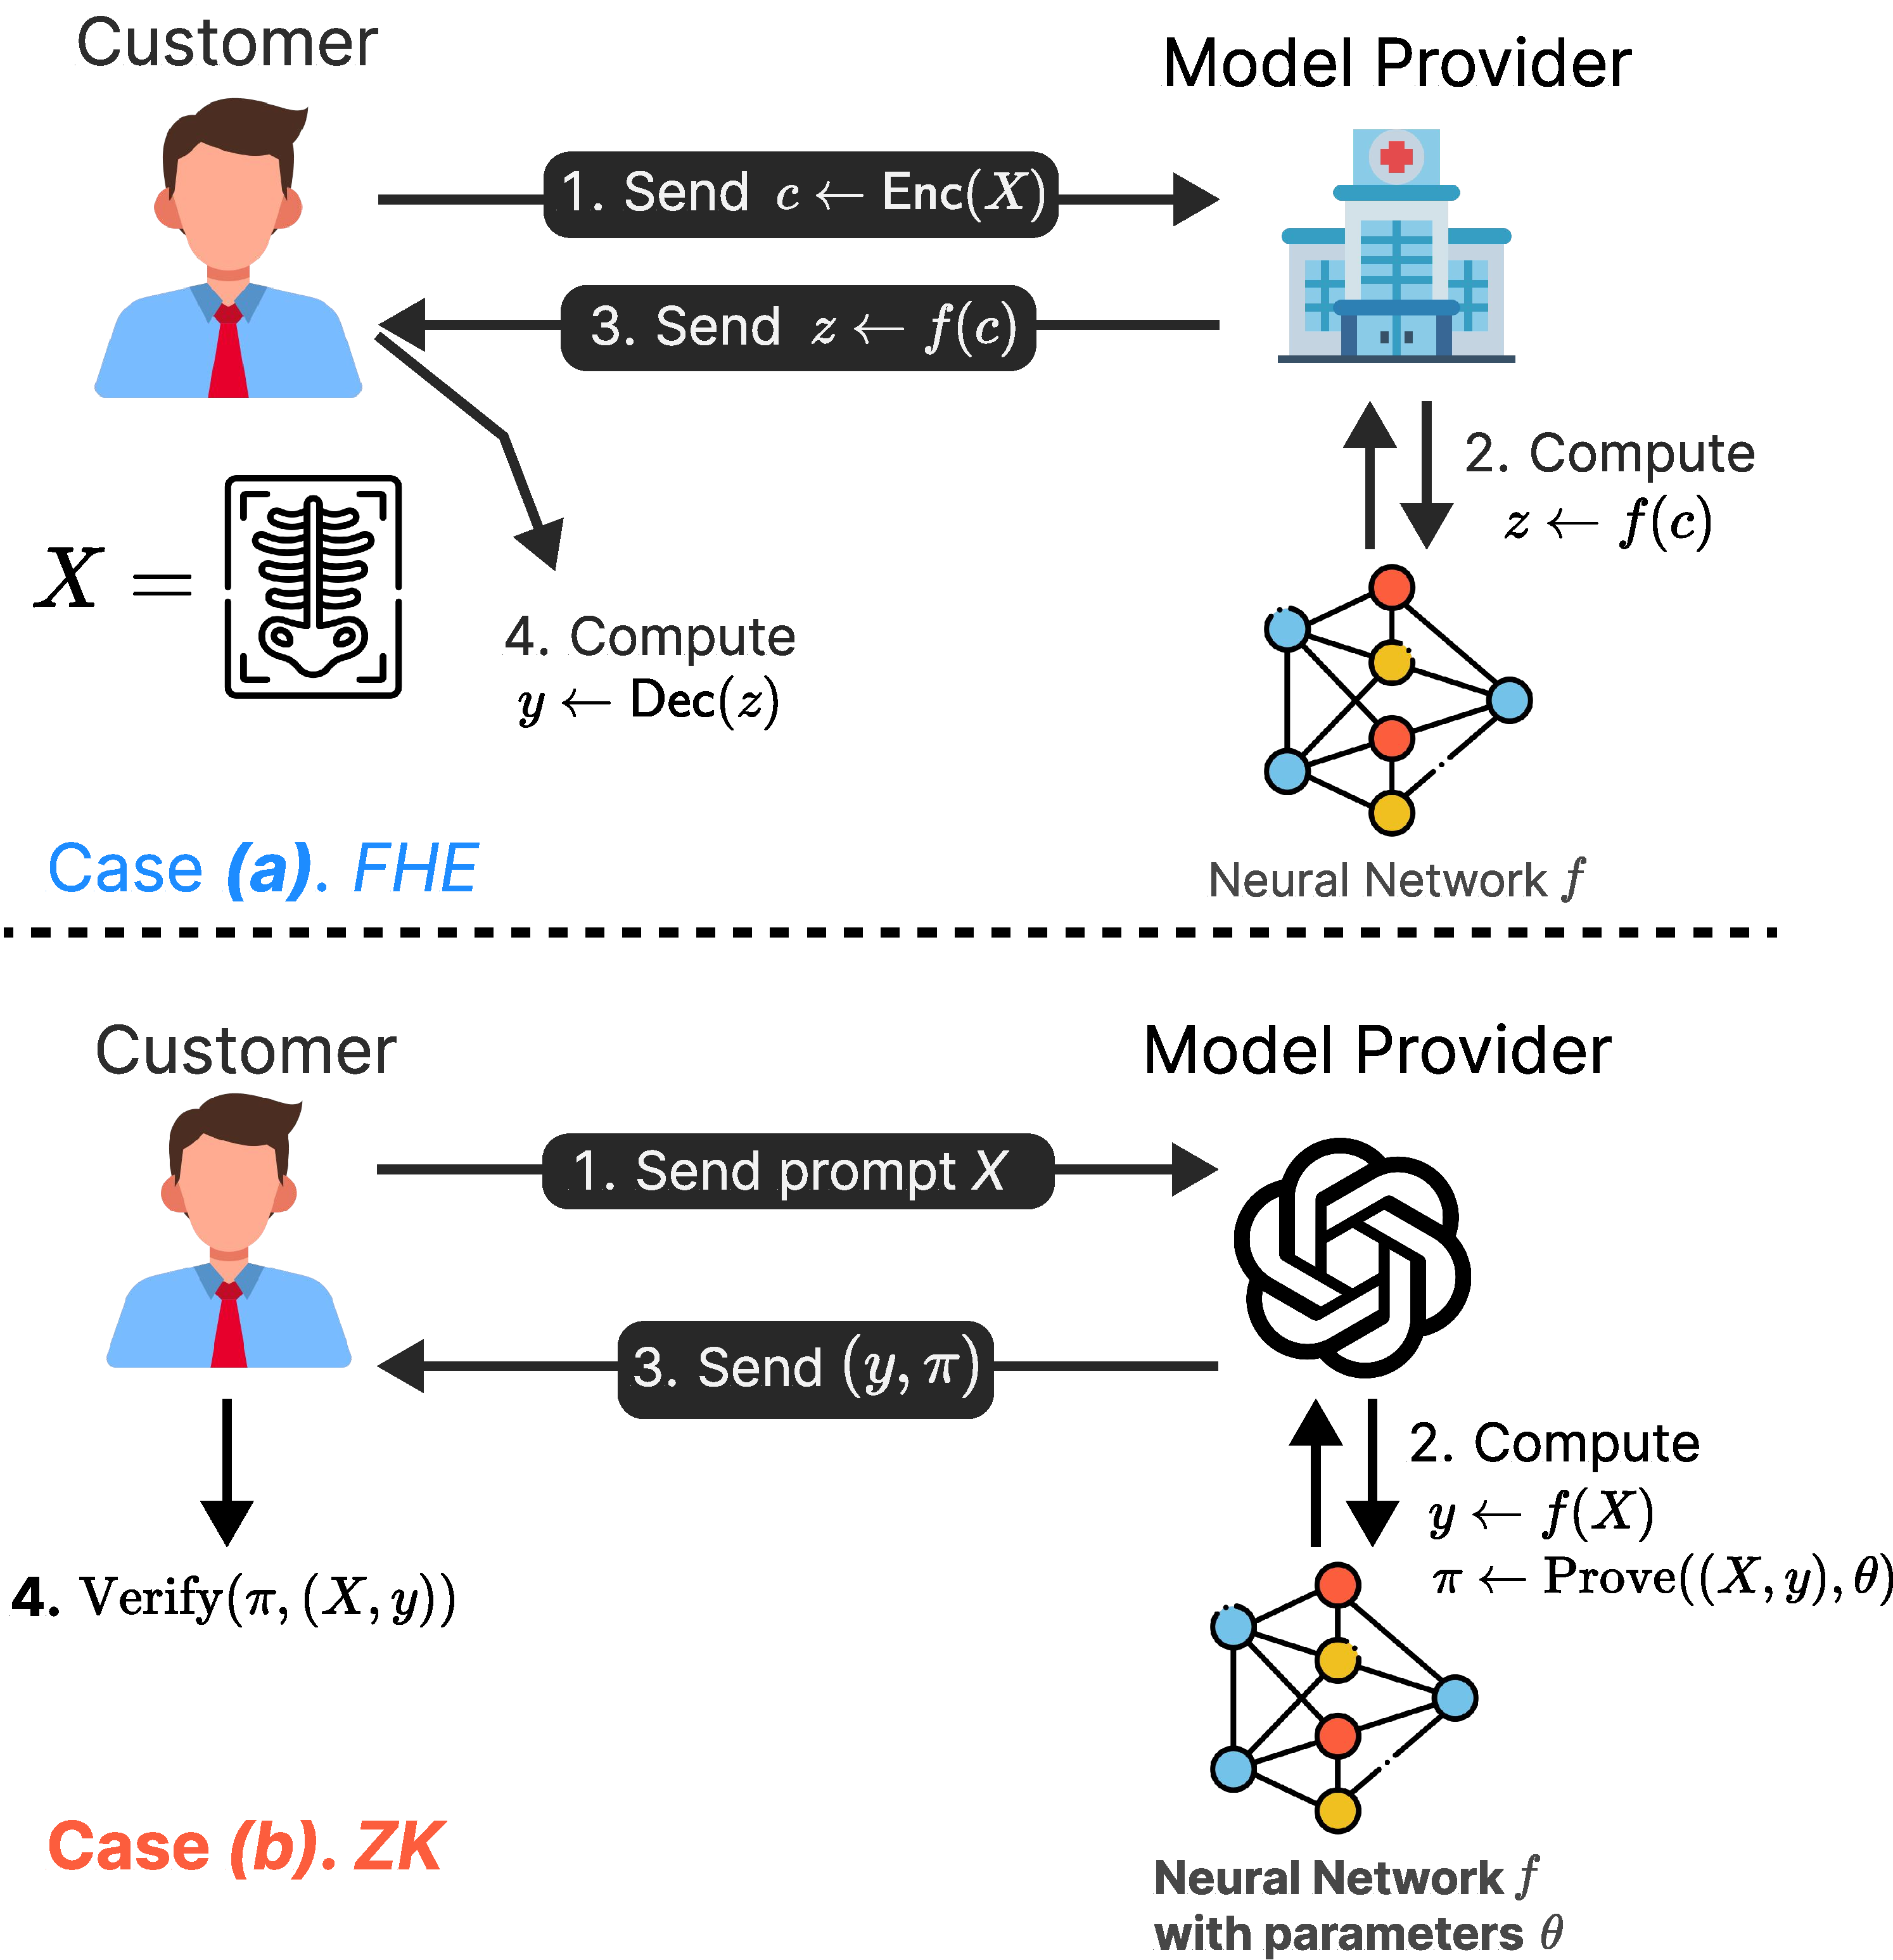
\includegraphics[width=0.6\textwidth]{images/use-cases.pdf}
            \caption{Приклади використання нейронних мереж у сферах безпеки.}
            \label{fig:nn-attack}
        \end{figure}
    \end{frame}

    \begin{frame}{Безпека нейронних мереж}
        \begin{itemize}
            \item Як ми можемо надіслати вхід $x$ нейронній мережі $f$ без
            розкриття $x$? Наприклад, чи може людина з зображенням
            рентгенівського знімка $x$ надіслати його алгоритму $f$ для
            діагностики, не показуючи знімок $x$ (див. \cite{cryptonets})?
            \item Чи можемо ми дійсно довіряти виходу нейронної мережі $y$?
            Інакшими словами, маючи вхід $x$, як ми можемо переконатись, що 
            дійсно $y = f(x)$ (див. \cite{nn-ezkl})? 
            \item Як ми можемо довести, що $f$ дійсно була натренована на
            неконфідеційних даних (див. \cite{zk-training})? Чи можемо ми
            тренувати нейронну мережу на зашифрованому наборі даних
            (див. \cite{fhe-training})?
        \end{itemize}

        \begin{block}{Зауваження}
            Першою та третьою задачами займається \textbf{гомоморфне шифрування}
            (FHE), а другою --- \textbf{доведення нульового знання для
            алгоритмів машинного навчання} (ZKML).
        \end{block}
    \end{frame}

    \section[Інструменти]{Інструменти}

    \subsection{Гомоморфне шифрування}

    \begin{frame}{Гомоморфне шифрування}
        \begin{itemize}
            \item Гомоморфне шифрування --- це шифрування, що дозволяє
            виконувати обчислення над зашифрованими даними без їх
            розшифрування.
            \item Це означає, що ми можемо виконувати обчислення на
            зашифрованих даних, не знаючи самих даних.
        \end{itemize}
        
        \begin{figure}
            \centering
            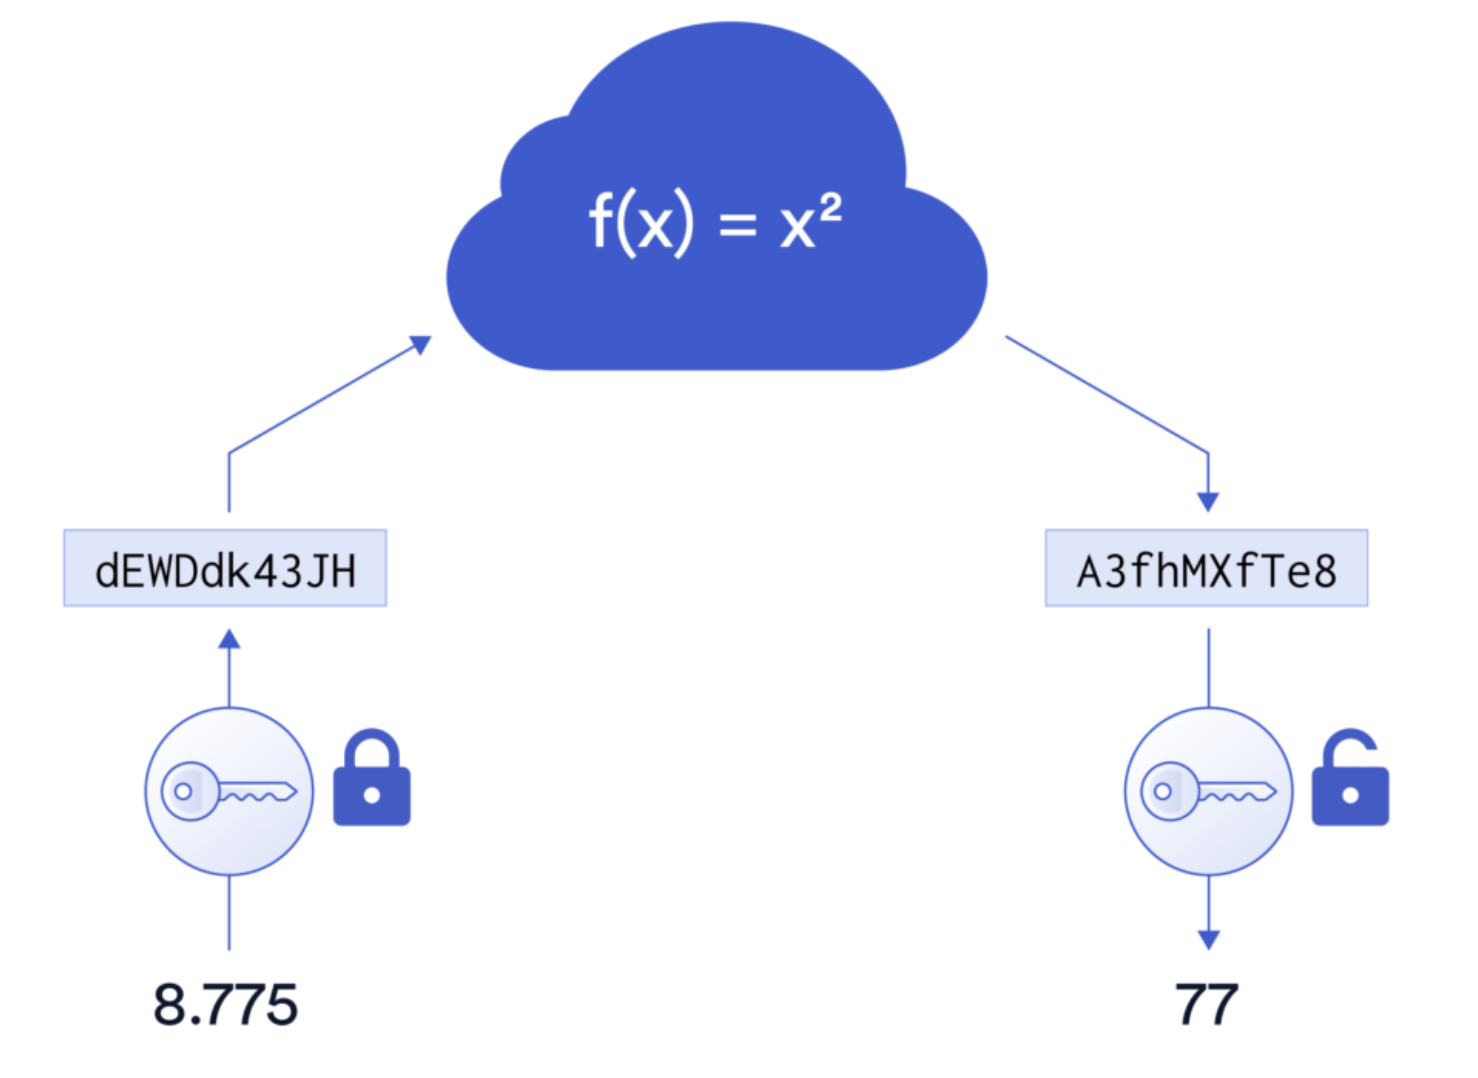
\includegraphics[width=0.5\textwidth]{images/fhe.png}
            \caption{Ілюстрація гомоморфного шифрування. Взято з
            \url{https://chain.link/education-hub/homomorphic-encryption}.}
            \label{fig:fhe}
        \end{figure}
    \end{frame}

    \begin{frame}{Гомоморфне шифрування: Означення}
        \begin{definition}[Схема повністю гомоморфного шифрування] \textbf{Схема
        повністю гомоморфного шифрування} (FHE) — це алгоритми
        $(\mathrm{KeyGen}, \mathrm{Enc}, \mathrm{Dec}, \mathrm{Eval})$: 
        \begin{itemize} 
            \item $\mathrm{KeyGen}(1^{\lambda}) \to
        (\mathsf{sk},\mathsf{ek})$: З огляду на параметр безпеки $\lambda \in
        \mathbb{N}$, видає секретний ключ $\mathsf{sk}$, який зберігається в
        таємниці користувачем, та публічний ключ для обчислень $\mathsf{ek}$.
            \item $\mathrm{Enc}(\mathsf{sk},\mu) \to c$: З огляду на секретний
            ключ $\mathsf{sk}$ та повідомлення $\mu$, видає шифротекст $c$.
            \item $\mathrm{Dec}(\mathsf{sk},c) \to \mu$: З огляду на секретний
            ключ $\mathsf{sk}$ та шифротекст $c$, видає повідомлення $\mu$.
            \item $\mathrm{Eval}(\mathsf{ek},f,c_1,\ldots,c_{\ell}) \to
            \widetilde{c}$: З огляду на ключ для обчислень $\mathsf{ek}$,
            функцію $f \in \mathcal{F}$ з підтримуваного класу функцій
            $\mathcal{F}$, та шифротексти $c_1,\ldots,c_{\ell}$, видає
            шифротекст результату застосування функції $f$ до відповідних
            відкритих значень.
        \end{itemize} 
    \end{definition}
    \end{frame}

    \begin{frame}{Гомоморфне шифрування: Властивості}
        \textcolor{blue!80!black}{\textbf{Коректність:}} для будь-якої
        допустимої функції $f \in \mathcal{F}$ та вхідних повідомлень
        $\mu_1,\dots,\mu_{\ell}$, маємо
        \begin{equation*}
            \small\text{Pr}\left[ \mathsf{Dec}(\mathsf{sk},\widetilde{c}) = f(\mu_1,\dots,\mu_{\ell}) \; \middle| \; \begin{matrix}
                (\mathsf{sk},\mathsf{ek}) \gets \mathsf{KeyGen}(1^{\lambda}) \\
                c_j \gets \mathsf{Enc}(\mathsf{sk},\mu_j), j \in [\ell], \\
                \widetilde{c} \gets \mathsf{Eval}(\mathsf{ek},f,c_1,\dots,c_{\ell})
            \end{matrix} \right] \geq 1 - \mu(\lambda),
        \end{equation*}

        де $\mu(\lambda)$ є нехтовною функцією: $\lim_{\lambda \to
        \infty}\mu(\lambda)\lambda^{\gamma} = 0$ для всіх $\gamma$.

        \textcolor{purple}{\textbf{Семантична безпека:}} для всіх повідомлень
        $\mu_0,\mu_1$ виконується
        \begin{equation*}
            \small\left\{ (\mathsf{ek},c_0): \begin{matrix}
                (\mathsf{sk},\mathsf{ek}) \gets \mathsf{KeyGen}(1^{\lambda}) \\
                c_0 \gets \mathsf{Enc}(\mathsf{sk},\mu_0)
            \end{matrix} \right\} \approx_C \left\{ (\mathsf{ek},c_1): \begin{matrix}
                (\mathsf{sk},\mathsf{ek}) \gets \mathsf{KeyGen}(1^{\lambda}) \\
                c_1 \gets \mathsf{Enc}(\mathsf{sk},\mu_1)
            \end{matrix} \right\}
        \end{equation*}
        Тут $\approx_C$ означає обчислювальну еквівалентність.

    \end{frame}

    \subsection{Доведення нульового знання}

    \begin{frame}{Доведення нульового знання}
        \begin{itemize}
            \item Доведення нульового знання --- це протокол, що дозволяє
            одній стороні (доказнику) довести іншій стороні (перевіряючому),
            що вона знає певну інформацію, не розкриваючи цю інформацію.
            \item Це означає, що доказник може довести перевіряючому, що він
            знає секрет, не розкриваючи сам секрет.
        \end{itemize}
        
        \begin{figure}
            \centering
            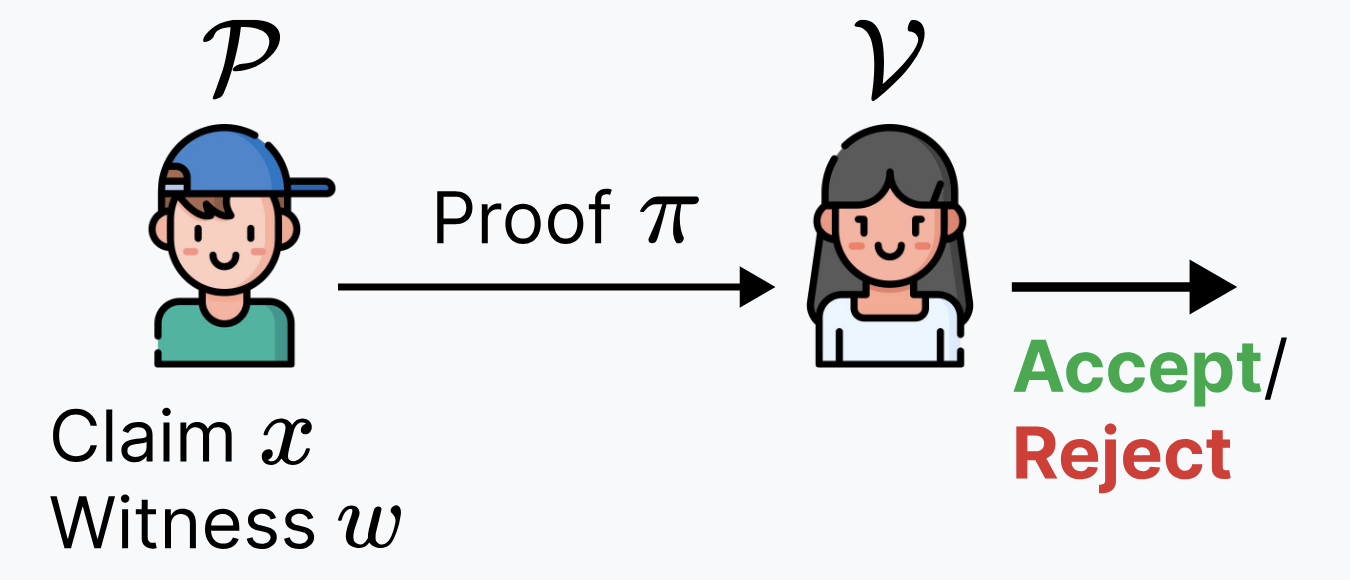
\includegraphics[width=0.8\textwidth]{images/zk.png}
            \caption{Ілюстрація доведення нульового знання.}
            \label{fig:zk}
        \end{figure}
    \end{frame}

    \begin{frame}{Доведення нульового знання: означення}
        \begin{definition}
            zk-SNARK — це протокол доведення з нульовим розголошенням (zero-knowledge proof system), 
            який дозволяє доводити знання свідка $\mathbbm{w}$ для твердження $\mathbbm{x}$ 
            у відношенні $\mathcal{R}$ без розголошення самого свідка. zk-SNARK складається з таких алгоритмів:
            \begin{itemize}
                \item $\mathrm{KeyGen}(1^{\lambda}) \to (\mathsf{pp},\mathsf{vp})$: 
                алгоритм генерації ключів, що створює параметри для доведення $\mathsf{pp}$ 
                та параметри для верифікації $\mathsf{vp}$ на основі параметра безпеки $\lambda \in \mathbb{N}$.
        
                \item $\mathrm{Prove}(\mathsf{pp}, \mathbbm{x}, \mathbbm{w}) \to \pi$: 
                алгоритм доведення, що генерує доказ $\pi$ для твердження $\mathbbm{x}$ 
                зі свідком $\mathbbm{w}$ на основі параметрів доведення $\mathsf{pp}$.
        
                \item $\mathrm{Verify}(\mathsf{vp}, \pi, \mathbbm{x}) \to \{0, 1\}$: 
                алгоритм перевірки, що перевіряє, чи доказ $\pi$ є дійсним для твердження $\mathbbm{x}$, 
                і повертає біт $1$, якщо доказ дійсний, і $0$ — інакше.
            \end{itemize}
        \end{definition}        
    \end{frame}

    \begin{frame}{Доведення нульового знання: властивості}
        \begin{itemize}
            \item \textcolor{blue!80!black}{\textbf{Коректність:}} для всіх
            $\mathbbm{x}$ та $\mathbbm{w}$ для яких $(\mathbbm{x}, \mathbbm{w})
            \in \mathcal{R}$ та $(\mathsf{pp},\mathsf{vp}) \gets
            \mathrm{KeyGen}(1^{\lambda})$,
            $\text{Pr}[\mathrm{Verify}(\mathsf{vp}, \pi, \mathbbm{x}) = 1] =
            1-\mu(\lambda)$, де доведення генерується як $\pi \gets
            \mathrm{Prove}(\mathsf{pp}, \mathbbm{x}, \mathbbm{w})$.
            \item \textcolor{purple}{\textbf{Непідробність:}} для параметрів
            $(\mathsf{pp},\mathsf{vp}) \gets \mathrm{KeyGen}(1^{\lambda})$ та
            $(\mathbbm{x},\mathbbm{w}) \gets
            \mathcal{A}(\mathsf{pp},\mathsf{vp})$ за умови $(\mathbbm{x},
            \mathbbm{w}) \not\in \mathcal{R}$, маємо
            $\text{Pr}[\mathrm{Verify}(\mathsf{vp}, \pi, \mathbbm{x}) = 1] =
            \mu(\lambda)$ для будь-якого поліноміально-випадкового алгоритму
            $\mathcal{A}$, що генерує $\pi$.
            \item \textcolor{green!60!black}{\textbf{Нульове знання:}} якщо
            $\mathrm{Verify}(\mathsf{vp}, \pi, \mathbbm{x}) = 1$, то не існує
            алгоритму, який може дістати інформацію про $\mathbbm{w}$ з $\pi$ та
            $\mathbbm{x}$ зі значною перевагою.
            \item \textcolor{orange!80!black}{\textbf{Ефективність:}} зазвичай,
            розмір доведення $|\pi| = \mathcal{O}_{\lambda}(\log^{\alpha} n,
            |\mathbbm{x}|)$ та час верифікації $T_{\mathcal{V}} =
            \mathcal{O}_{\lambda}(\log^{\beta} n, |\mathbbm{x}|)$ (себто
            полілогарифмічна асимптотика) для деяких $\alpha,\beta$.
            
        \end{itemize}
    \end{frame}

    \begin{frame}{Арифметичні ланцюги}
        Так чи інакше, щоб працювати над гомоморфно зашифрованими даними або
        протоколами доведення нульового знання, нам потрібно мати
        \textbf{арифметичні ланцюги} --- це графи, що складаються з
        \textbf{вузлів} (операцій) та \textbf{проводів} (входів/виходів), які
        представляють обчислення над елементами (зазвичай скінченного) поля
        $\mathbb{F}_p$.

        \begin{figure}
            \centering
            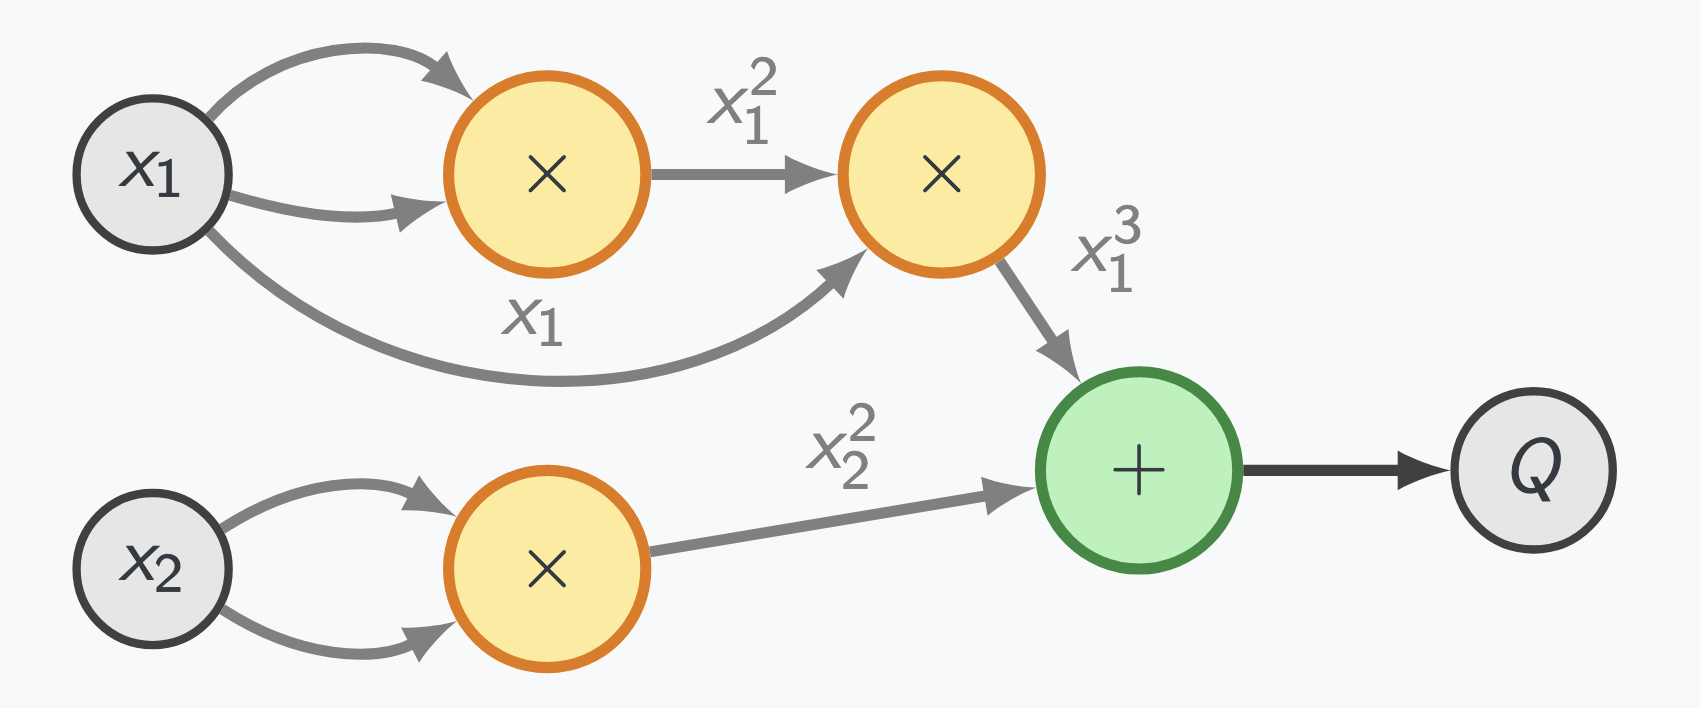
\includegraphics[width=0.75\textwidth]{images/circuits.png}
            \caption{Приклад арифметичного ланцюга для функції $x_1^3 + x_2^2$.}
            \label{fig:arithmetic-circuit}
        \end{figure}
    \end{frame}

    \begin{frame}{Нейронні мережі як арифметичні ланцюги}
        \begin{itemize}
            \item Усі обчислення нейронної мережі (котрі проводяться 
            над дійсним полем $\mathbb{R}$) можуть бути представлені
            арифметичними ланцюгами, що складаються з операцій
            \textbf{додавання} та \textbf{множення} над певним 
            \textbf{полем} $\mathbb{F}_p$.
            \item Проте, кількість вузлів в такому графі дуже критично 
            збільшує час на доведення та часто верифікації доведень для 
            ZK та сильно збільшує час на обчислення для FHE (а іноді і накопичує 
            помилки при обчисленнях).
            \item Тому, ми можемо спробувати зменшити кількість вузлів
            в графі, зберігаючи при цьому точність нейронної мережі.
            \item Це можна зробити за допомогою \textbf{активаційно-ефективних
            архітектур нейронних мереж}, які зберігають точність нейронної
            мережі, але зменшують кількість вузлів в графі за рахунок
            використання меншої кількості активаційних функцій.
        \end{itemize}    
    \end{frame}

    \section{Активаційно-ефективні архітектури нейронних мереж}
    \begin{frame}{Активаційні функції}
        \begin{table}[H]
            \centering
            \begin{tabular}{cccc}
                \hline
                \textbf{Назва} & \textbf{Формула} & \textbf{Де використовується?} \\
                \hline
                ReLU & $\max\{0,x\}$ & Дешева нелінійність \\
                $\text{LeakyReLU}_{\alpha}$ & $\max\{\alpha x,x\}$ & Дешева нелінійність \\
                Sigmoid $\sigma(x)$ & $\frac{1}{1+e^{-x}}$ & Бінарна класифікація \\
                Tanh & $\frac{1-e^{-2x}}{1+e^{-2x}}$ & Бінарна класифікація \\
                Softmax & $\left\{e^{x_i}/\sum_{j\in [n]}e^{x_j}\right\}_{i \in [n]}$ & Мультикласифікація \\
                Swish & $x\sigma(x)$ & Ефективна нелінійність \\
                \hline
            \end{tabular}
            \caption{Найбільш поширені активаційні функції.}
            \label{table:activations}
        \end{table}

        \begin{alertblock}{Питання}
            Як реалізувати такі активаційні функції, як ReLU, LeakyReLU, Sigmoid,
            Tanh, Softmax та Swish, у вигляді арифметичних ланцюгів, маючи лише 
            операції додавання та множення?
        \end{alertblock}
    \end{frame}

    \begin{frame}{Метод \#1: Апроксимація}
        \begin{block}{Ідея}
            Використовувати \textbf{апроксимацію} активаційних функцій
            поліномами, які можуть бути реалізовані у вигляді арифметичних
            ланцюгів.
        \end{block}

        \begin{table}[H]
            \centering
            \begin{tabular}{cccc}
                \hline
                \textbf{Назва} & \textbf{Апроксимація} \\
                \hline
                ReLU & $0.47 + 0.5x + 0.09x^2$ \\
                Tanh & $0.51x - 0.04x^3 + 0.0011x^5$ \\
                Swish & $0.24 + 0.5x + 0.1x^2$\\
                \hline
            \end{tabular}
            \caption{Апроксимація поширених активаційних функцій поліномами.}
            \label{table:activations-appr}
        \end{table}
    \end{frame}

    \begin{frame}{Проблеми}
        \begin{alertblock}{Проблеми}
            \begin{itemize}
                \item Зазвичай, гарна апроксимація лише на певному відрізку, отже 
                погіршується точність обчислень.
                \item А якщо тренувати модель на активаціях, що задані цими
                поліномами? Тоді не виконується теорема універсальної
                апроксимації, а отже емпірично губиться точність.
                \item Отже, краще використовувати активації як є.
            \end{itemize}
        \end{alertblock}

        Будь-які експоненти не можуть бути реалізовані у вигляді
        арифметичних ланцюгів, тому що вони не є поліномами. Тому,
        \begin{itemize}
            \item Ми використовуємо тільки $\mathsf{ReLU}$ та
            $\mathsf{LeakyReLU}$ з параметром $\alpha=2^{-d}$, що 
            є степінню двійки.
            \item Замість $\mathsf{Softmax}$ або $\mathsf{Sigmoid}$ (якщо це
            активація в кінці), використовуємо функції максимуму.
        \end{itemize}
    \end{frame}

    \begin{frame}{Вартість ReLU}
        \begin{lemma}
            Обчислення $\mathsf{ReLU}$ вартує $b+1$ множень в арифметичному
            ланцюзі, де $b = \lceil \log_2 \mathbb{F}\rceil$ --- кількість бітів в
            елементах поля $\mathbb{F}$.
        \end{lemma}

        \textbf{Доведення.} Треба розкласти $x$ на двійкові
        компоненти $x = \sum_{i=0}^{b-1} x_i 2^i$ та переконатись, що 
        $x_i \in \{0,1\}$. Щоб перевірити бінарність $x_i$, достатньо 
        зробити $b$ множень $x_i(1-x_i)=0$. Далі якщо $x_j$ позначає 
        знак числа, то достатньо обчислити $x_jx$, що вартує $1$
        множення. Отже, загальна вартість $b+1$ множень.

        \textcolor{gray!50!black}{\textbf{Коментар.}} Зазвичай додавання та
        множення на константу --- дешева операція, тому не будемо її
        враховувати.
    \end{frame}

    \begin{frame}{Повнозв'язаний шар}
        Нехай $\boldsymbol{x} \in \mathbb{F}^m$ --- вхідний вектор, $W \in
        \mathbb{F}^{n \times m}$ --- матриця ваг, $\boldsymbol{b} \in \mathbb{F}^n$ ---
        вектор зсувів, $\boldsymbol{y} \in \mathbb{F}^n$ --- вихідний вектор. Тоді
        \begin{equation*}
            \boldsymbol{y} = \sigma(W \boldsymbol{x} + \boldsymbol{b}).
        \end{equation*}

        \begin{block}{Вартість}
            \begin{itemize}
                \item $mn$ множень для обчислення $\boldsymbol{W}\boldsymbol{x}+\boldsymbol{b}$.
                \item $nb$ множень для обчислення $\sigma(\cdot)$.
            \end{itemize}
            Отже, загальна вартість --- $n(m+b)$ множень. Чи можна краще?
        \end{block}
    \end{frame}

    \begin{frame}{Encoder-Decoder Шар}
        \begin{block}{Encoder-Decoder Шар}
            \textbf{Шар Encoder–Decoder} між $n$ нейронами на вході та $m$
нейронами на виході з $h$ прихованими одиницями визначається наступним чином.
Нехай $E \in \mathbb{F}^{n \times h}$ — матриця енкодера та $D \in \mathbb{F}^{h
\times m}$ — матриця декодера. Тоді:
\begin{equation*}
    f(\boldsymbol{x}; D, E) := D \sigma(E\boldsymbol{x})
\end{equation*}
        \end{block}

        \begin{figure}
            \centering
            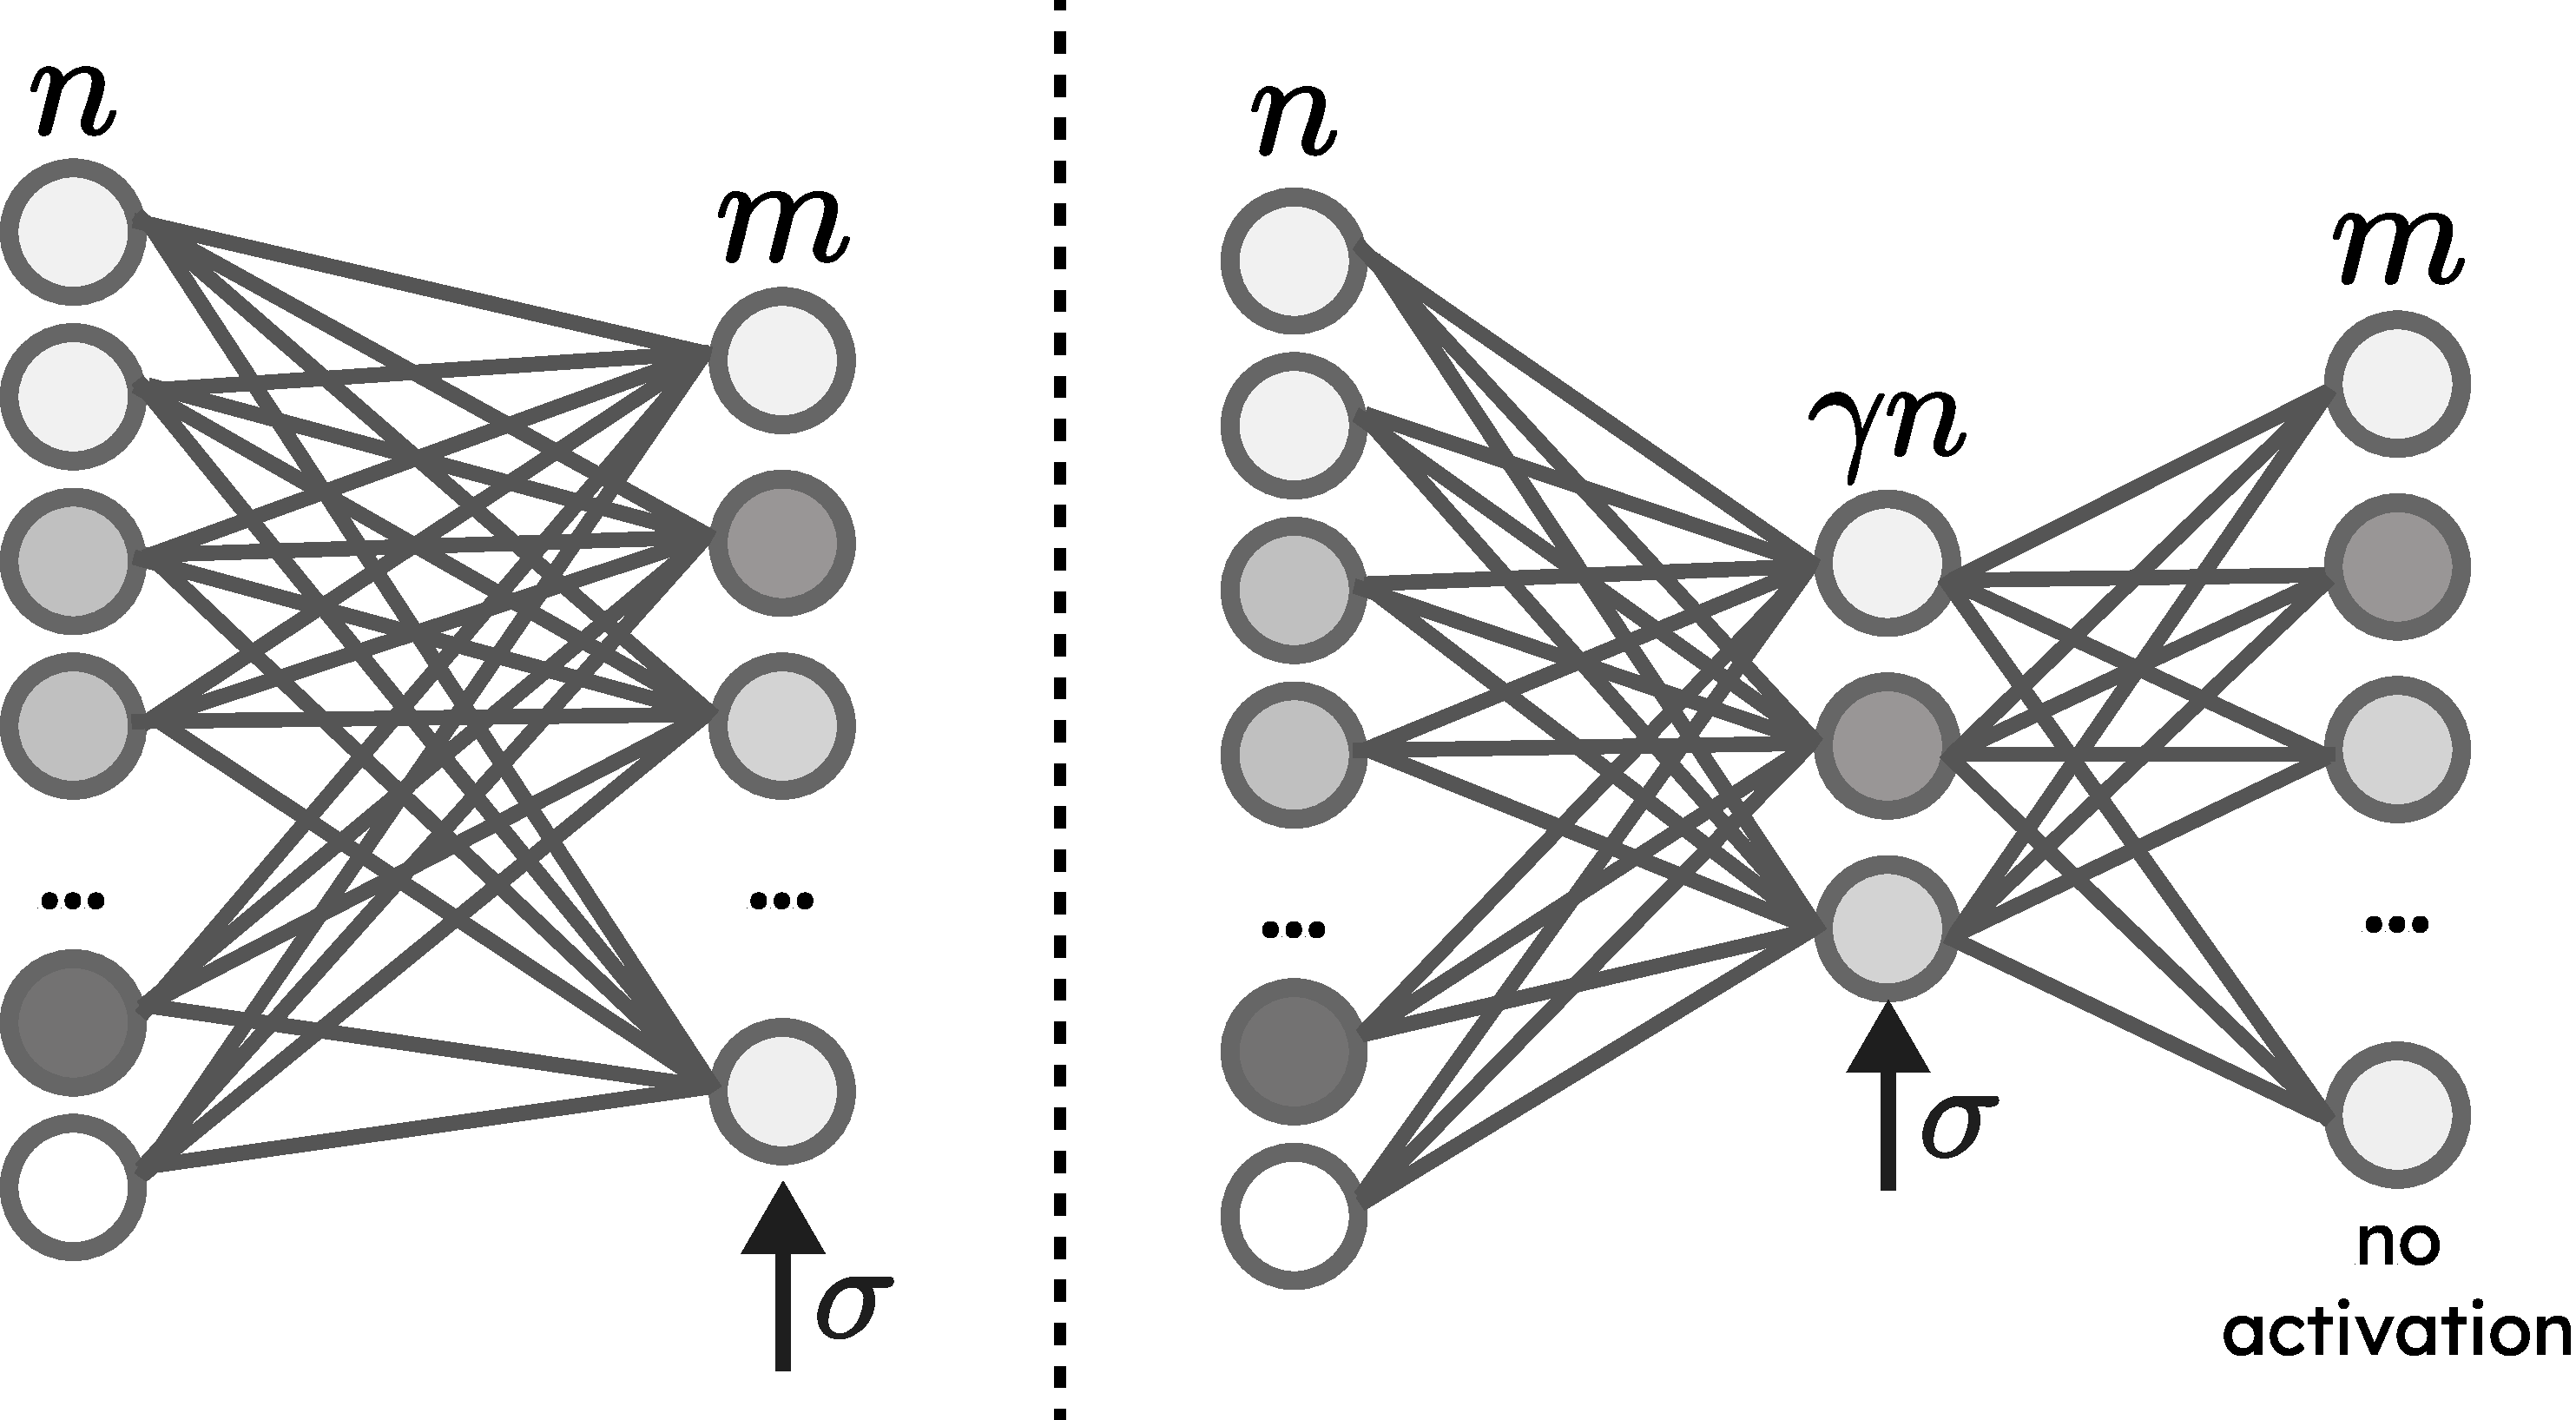
\includegraphics[width=0.6\textwidth]{images/ed.pdf}
            \caption{Encoder-Decoder Шар.}
            \label{figure:encoder-decoder}
        \end{figure}
    \end{frame}

    \begin{frame}{Переваги Encoder-Decoder Шару}
        \begin{lemma}
            Складність forward-pass шару дорівнює $\mathcal{O}(h(n + m +
            b))$ (на відміну від $O(n(m + b))$).
        \end{lemma}

        \begin{example}
            Припустимо, що $n = 1000$, $m = 10000$, а $h = 10$. Нехай
        розмірність поля дорівнює $b = 254$. Тоді складність прямого проходу через
        нейронну мережу з одним шаром становить: $10000(1000+254)\approx 10^7$. Натомість,
        складність прямого проходу через нейронну мережу з шаром Encoder-Decoder
        дорівнює: $10(1000+10000+254)\approx 10^5$. Це дає \textbf{зменшення в 100 разів}, що є
        суттєвим!
        \end{example}
    \end{frame}

    \begin{frame}{Реалізація}
        \begin{figure}
            \centering
            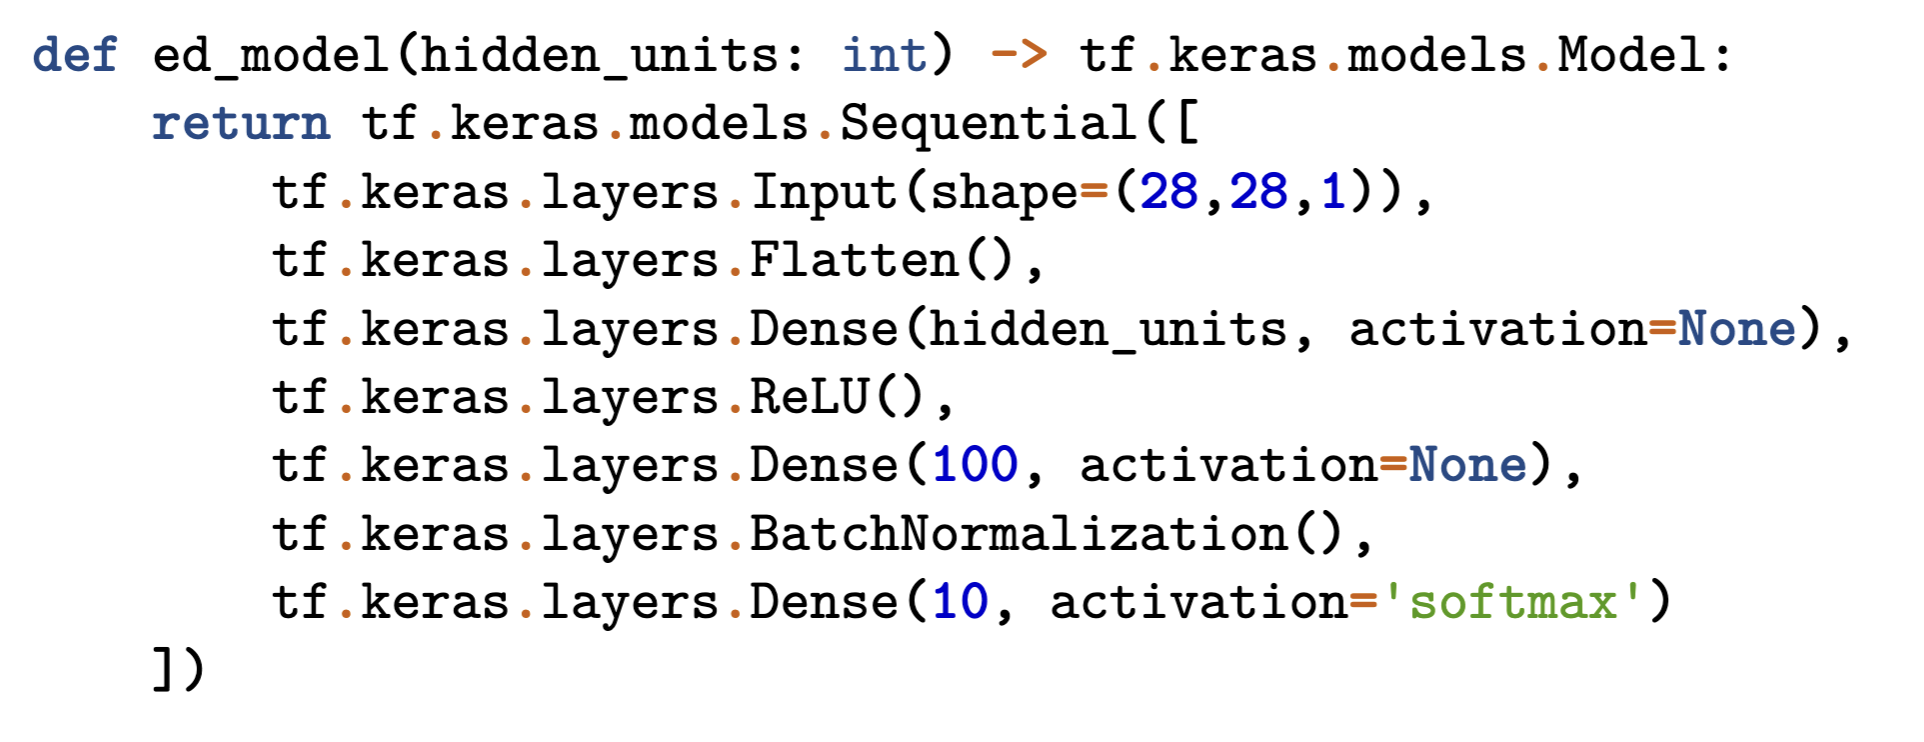
\includegraphics[width=\textwidth]{images/code.png}
            \caption{Реалізація Encoder-Decoder Моделі.}
            \label{figure:encoder-decoder}
        \end{figure}
    \end{frame}

    \begin{frame}{Датасет}
        \begin{figure}
            \centering
            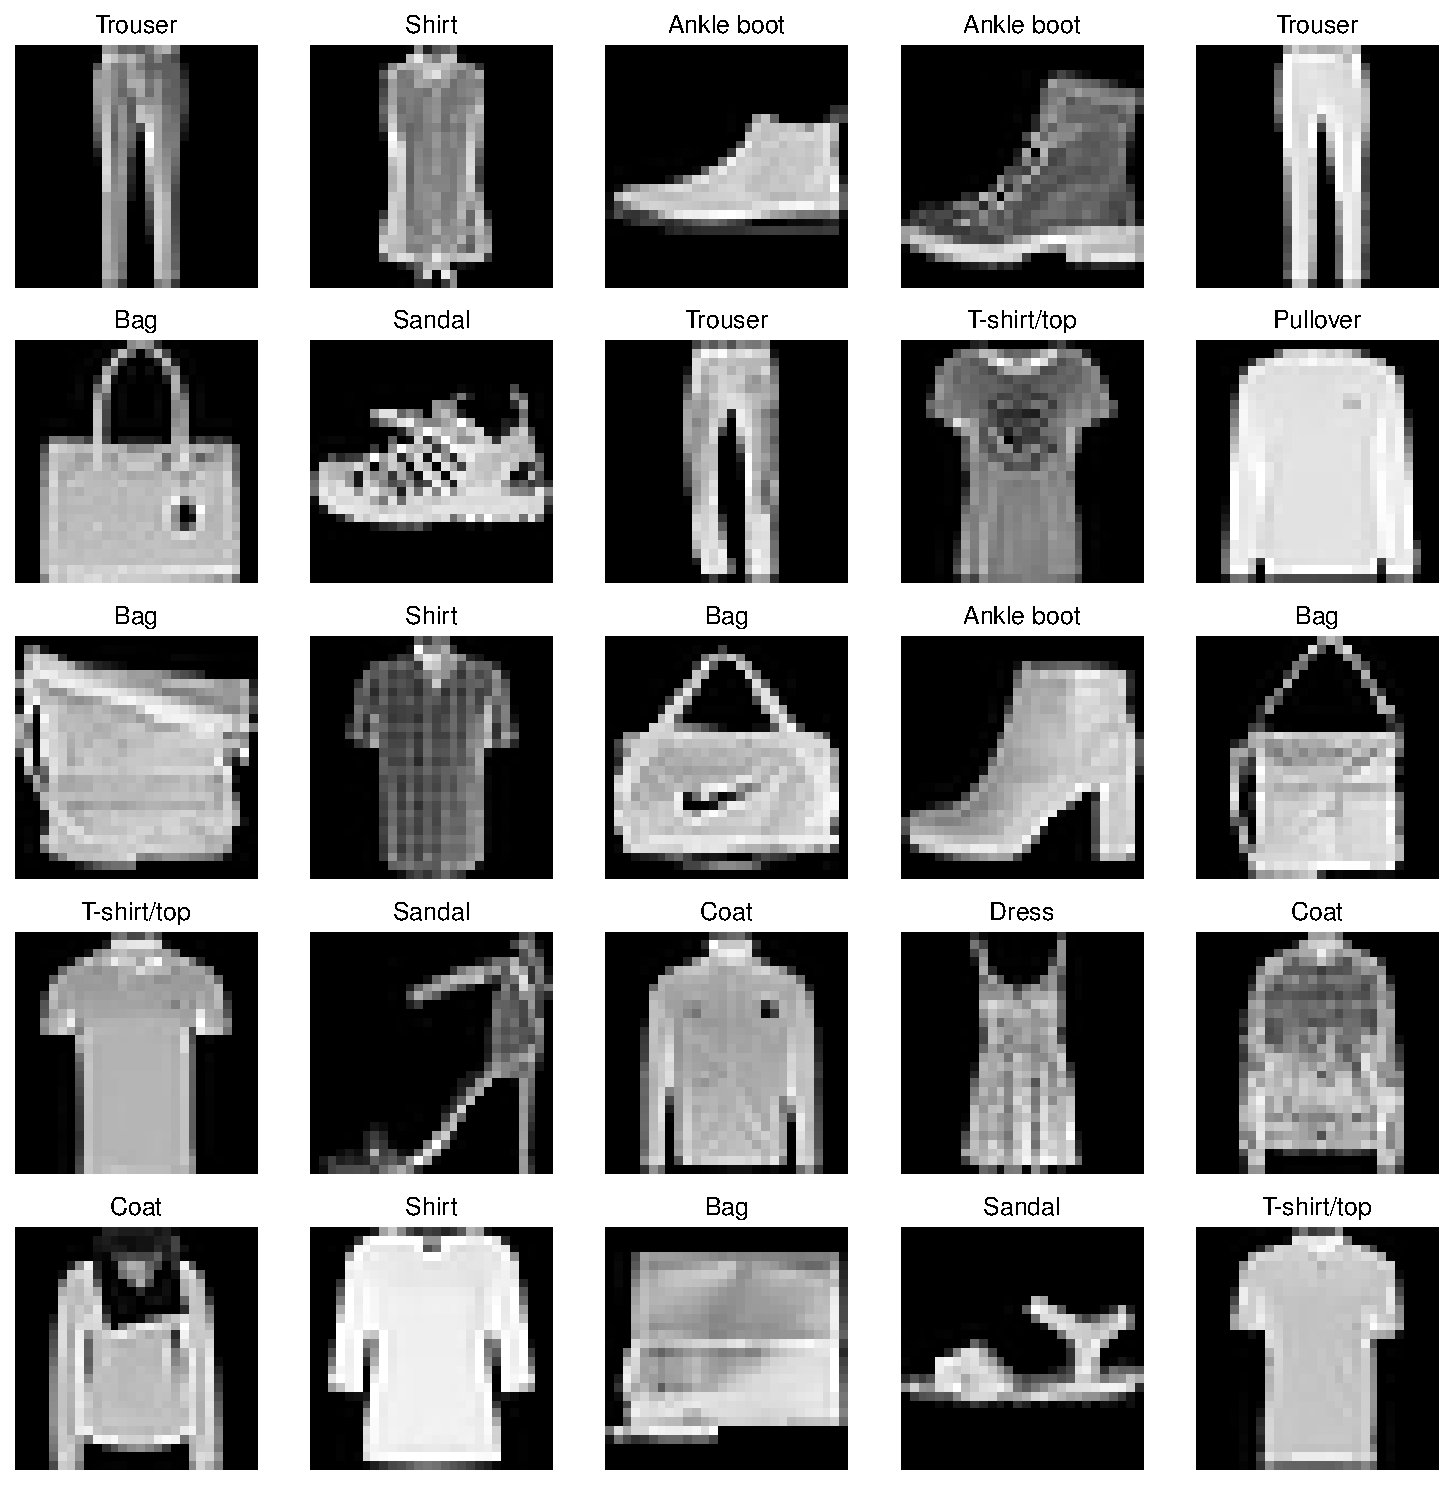
\includegraphics[width=0.6\textwidth]{images/fashion_mnist_grid.pdf}
            \caption{Ми використовували Fashion-MNIST датасет \cite{fashion-mnist}.}
            \label{figure:fashion-mnist}
        \end{figure}
    \end{frame}

    \begin{frame}{Графік точності від фактору стискання}
        \begin{figure}
            \centering
            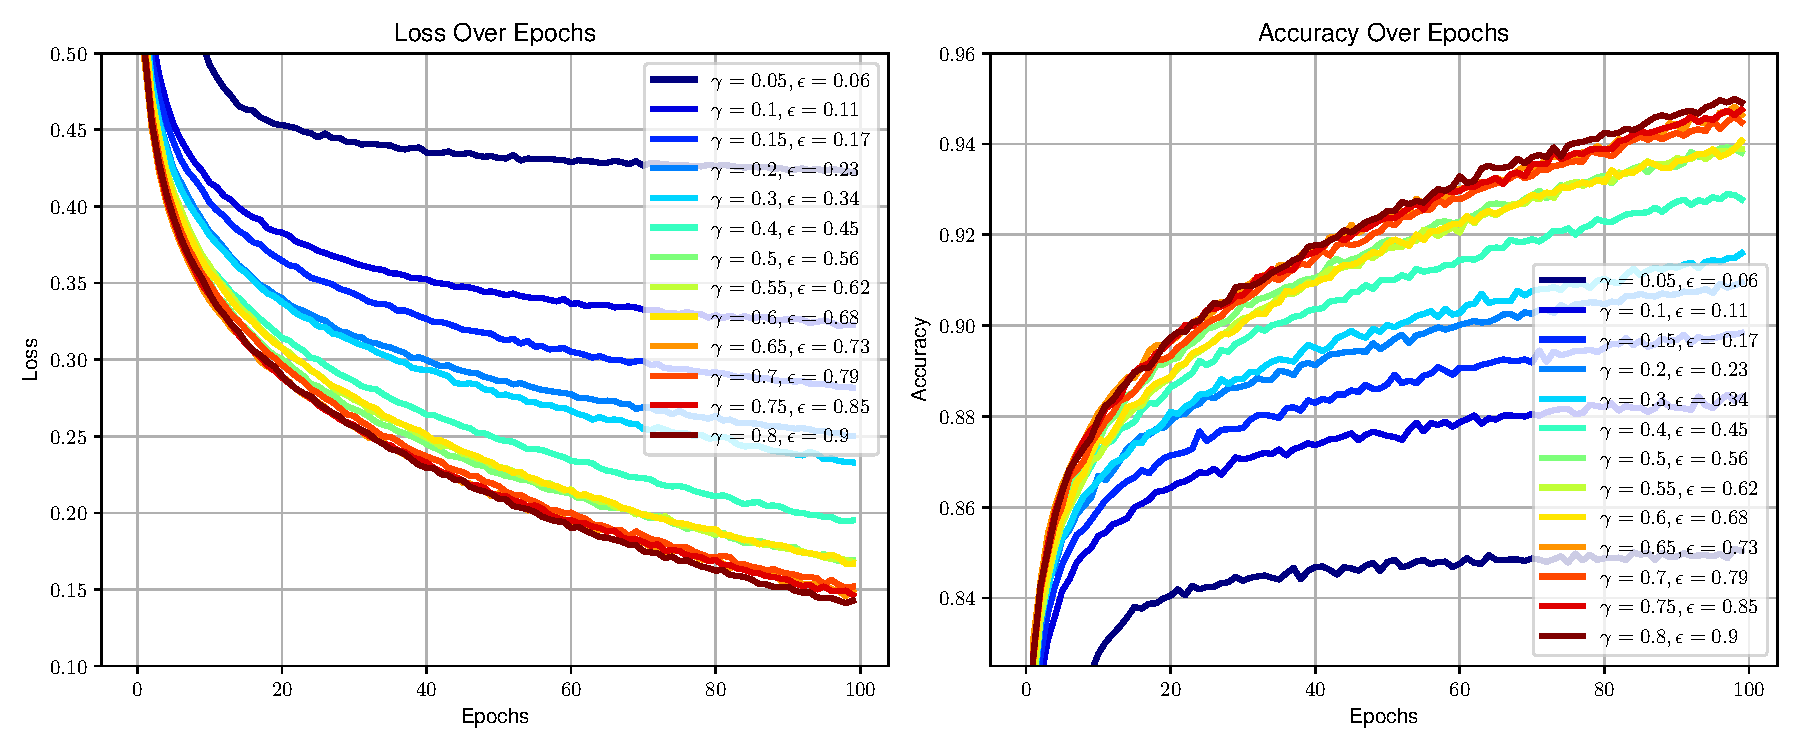
\includegraphics[width=\textwidth]{images/accuracy_loss_over_epochs_3.pdf}
            \caption{Графік точності від фактору стискання.}
            \label{figure:encoder-decoder-graph}
        \end{figure}
    \end{frame}

    \begin{frame}{Графік точності від фактору стискання}
        \begin{figure}
            \centering
            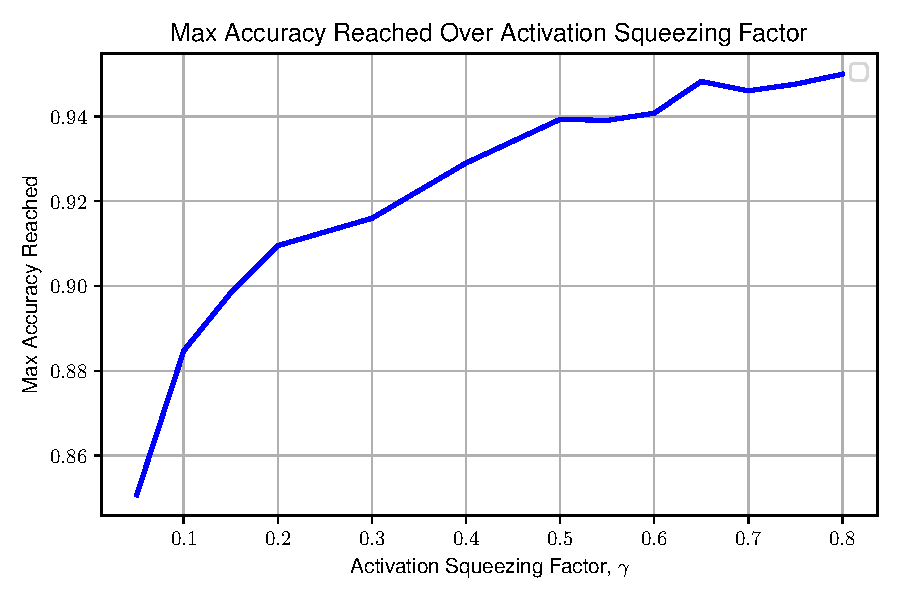
\includegraphics[width=0.9\textwidth]{images/max_accuracy_over_squeeze.pdf}
            \caption{Графік точності від фактору стискання.}
            \label{figure:encoder-decoder-graph}
        \end{figure}
    \end{frame}

    \begin{frame}[allowframebreaks]{Література}
        % This prints the bibliography on the slide
        \printbibliography
    \end{frame}

    \begin{frame}[plain, standout]
      \centering
      \LARGE
      \textbf{Дякую за Вашу Увагу!} \\
      
      \vspace{0.2cm} \Huge \ding{170} \large \\
    \end{frame}
\end{document}